\chapter{Detalles de Implementación y Experimentos}\label{chapter:implementation}

\section{Aplicación para la captura de señales}
	Para capturar las señales se utilizó una aplicación implementada en \textbf{Flutter} 2.10.15, con \textbf{dart} 2.16.2.
	Se utilizaron las bibliotecas \textbf{sensors\textunderscore plus} y \textbf{geolocator}, disponibles en \textbf{Flutter}, para obtener acceso
	a las lecturas del \textbf {acelerómetro}, \textbf{giroscopio} y \textbf{GPS}. Para comenzar a realizar una captura se aprieta el botón
	de \emph{Start recorder} y a partir de ese momento la aplicación comienza a reflejar los valores que se obtienen de los sensores en la
	interfaz de usuario.\\
	\indent La aplicación muestra en tiempo real las lecturas de los distintos sensores, así como la velocidad en kilómetros por hora (km/h) y la
	duración de la captura que se está realizando en el momento (ver figura \ref{fig:6}).\\
	\indent Cuando se desea detener la grabación se presiona el botón \emph{Stop recorder}. Luego si se quiere exportar dicha grabación se puede
	hacer presionando el botón de \emph{Save record as} e introduciendo el nombre con el que se desea salvar dichar grabación (ver figura
	\ref{fig:7}). De esta forma se puede acceder a todas las grabaciones para posteriormente utilizarlas en el modelo de aprendizaje de máquinas.\\
	\indent Con el botón \emph{Mark anomaly} se pueden realizar marcas, de esta forma se salvan las coordenadas de latitud-longitud en un
	archivo de marcas. La aplicación tiene además un mapa donde se pueden visualizar datos de latitud-longitud previamente guardados.
	Estos se pueden cargar en la pestaña del mapa de la aplicación para poder visualizar dichas marcas en el mapa (ver figura \ref{fig:8}).
	De esta forma se pueden marcar los baches y verlos en un mapa.\\
	
	\begin{figure}[htb]
		\centering
		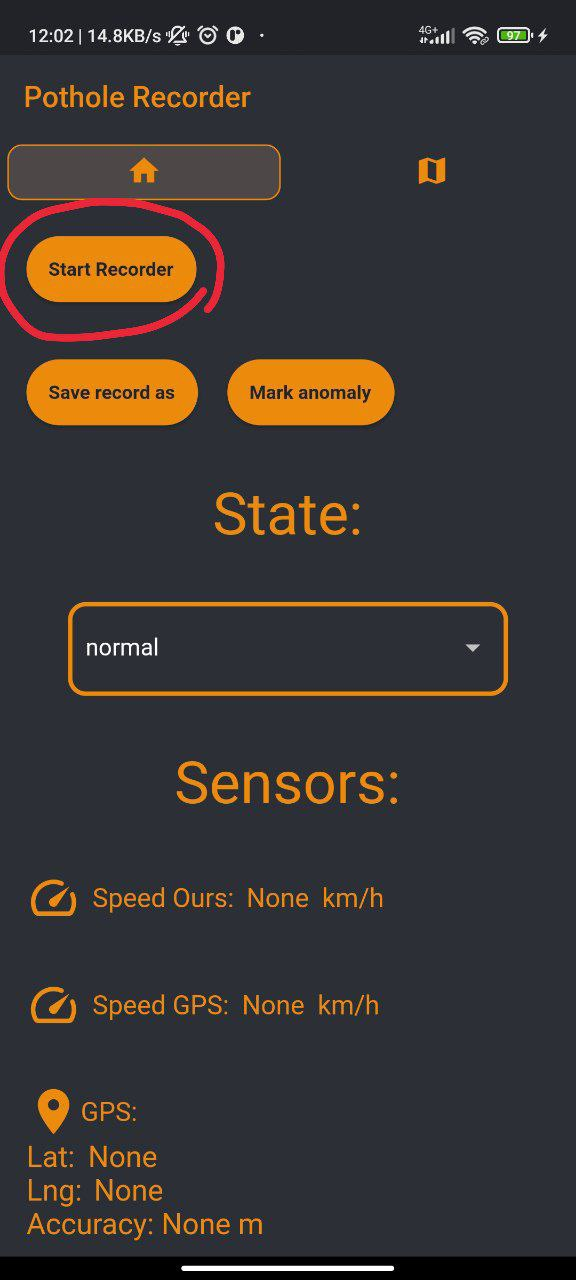
\includegraphics[scale = 0.2]{Graphics/apk_start_recording.jpg}
		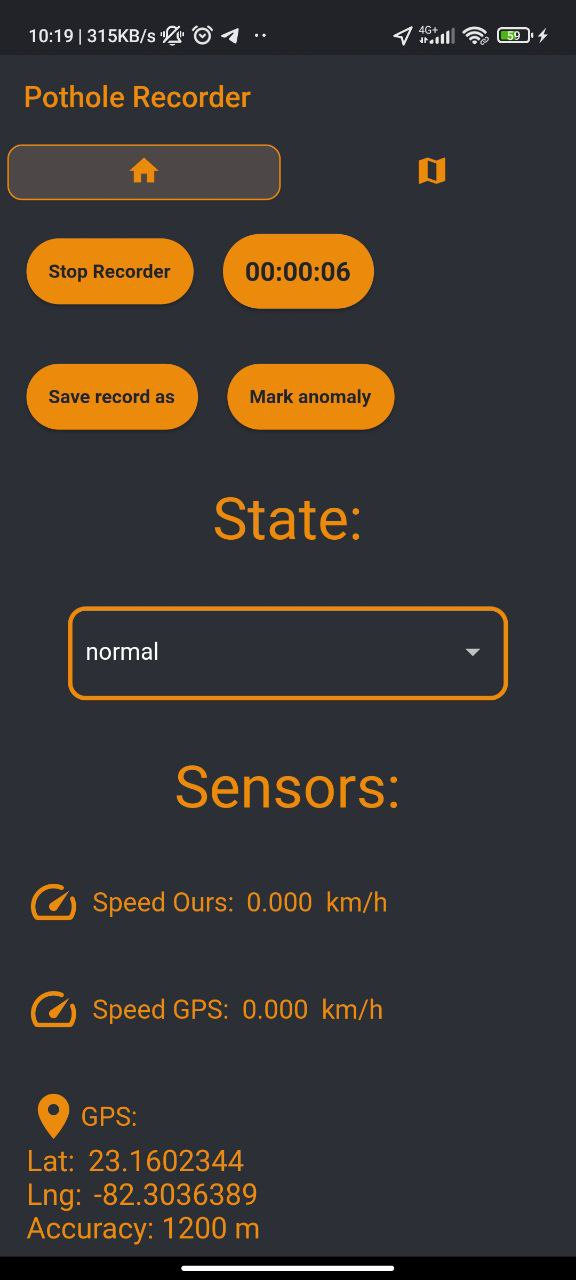
\includegraphics[scale = 0.2]{Graphics/apk_recording_ui.jpg}
		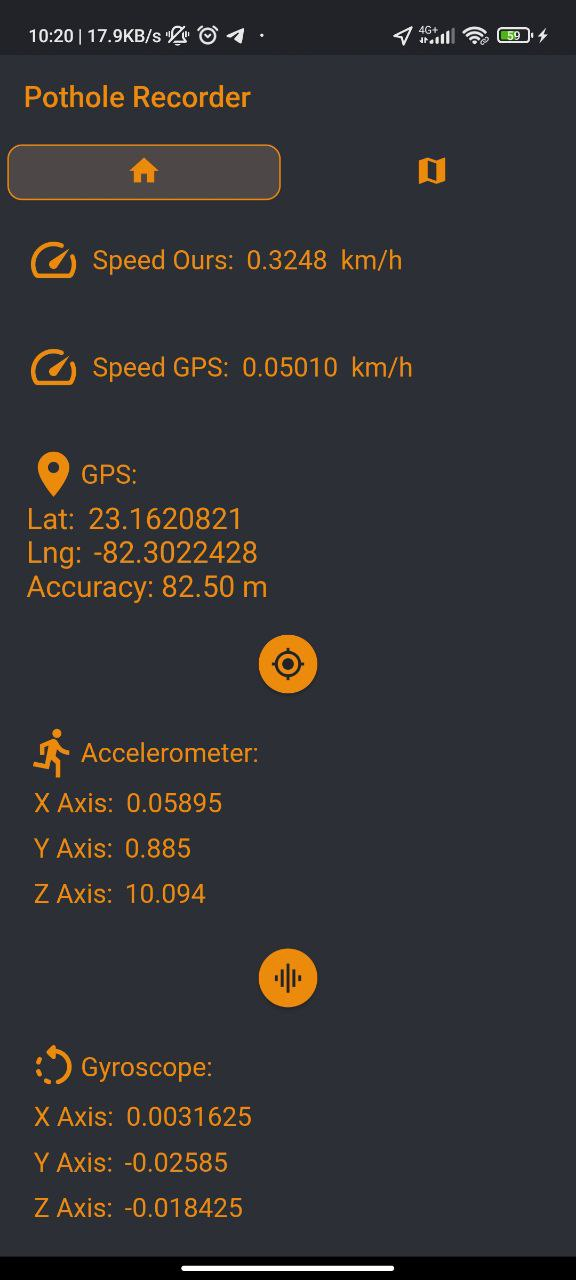
\includegraphics[scale = 0.2]{Graphics/apk_recording_sensors.jpg}
		\caption{Comenzar a grabar y lecturas reflejadas en la aplicación}
		\label{fig:6}
	\end{figure}
	\newpage

	\indent Es necesario dar permisos de escritura para salvar en el dispositivo móvil los archivos que se obtienen como resultado del 
	muestreo de los sensores, los archivos exportados y el archivo donde se almacenan las marcas que se realizan manualmente. Estos archivos
	se guardan en un directorio nombrado \textbf{Baches} en la raíz del almacenamiento interno del dispositivo móvil.\\
	\indent En esta carpeta hay otras 3 carpetas:

	\begin{itemize}
		\item \textbf{mark\textunderscore labels}: Donde se guardan las marcas.
		\item \textbf{sensors}: Donde se guarda el archivo temporal en el que se van guardando los datos que va recopilando la aplicación
			mientras está grabando.
		\item \textbf{exported} donde se guardan los archivos exportados.
	\end{itemize}

	Además, es necesario dar permisos de ubicación a la aplicación para que pueda acceder a los datos del \textbf{GPS}, latitud y longitud,
	en tiempo real.

	\begin{figure}[htb]
		\centering
		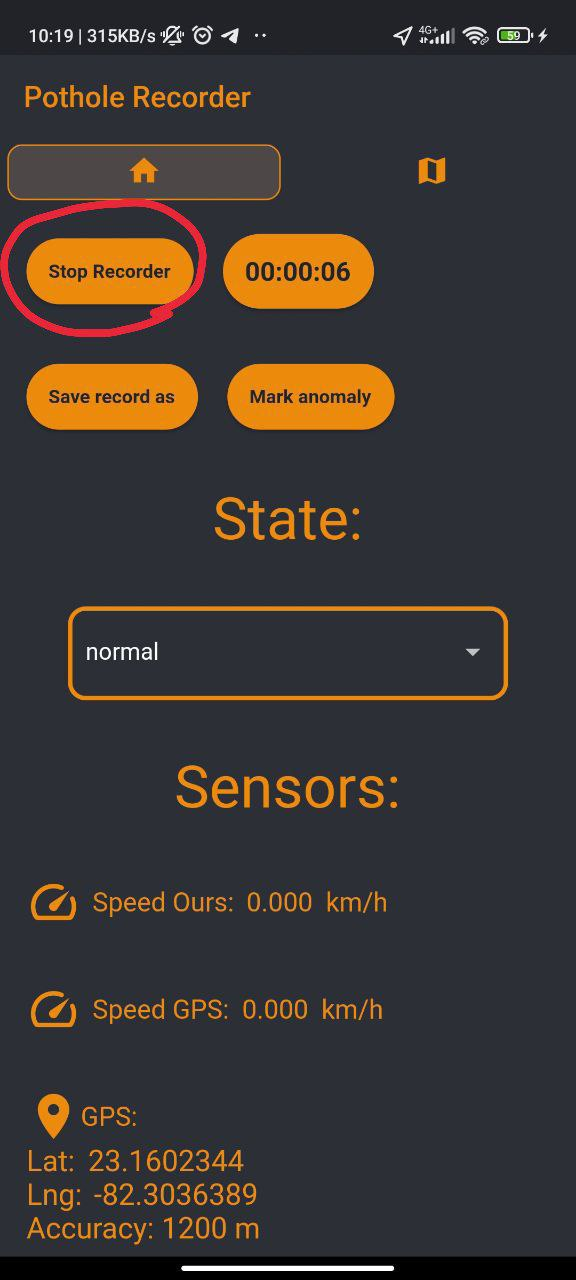
\includegraphics[scale = 0.175]{Graphics/apk_stop_recording.jpg}
		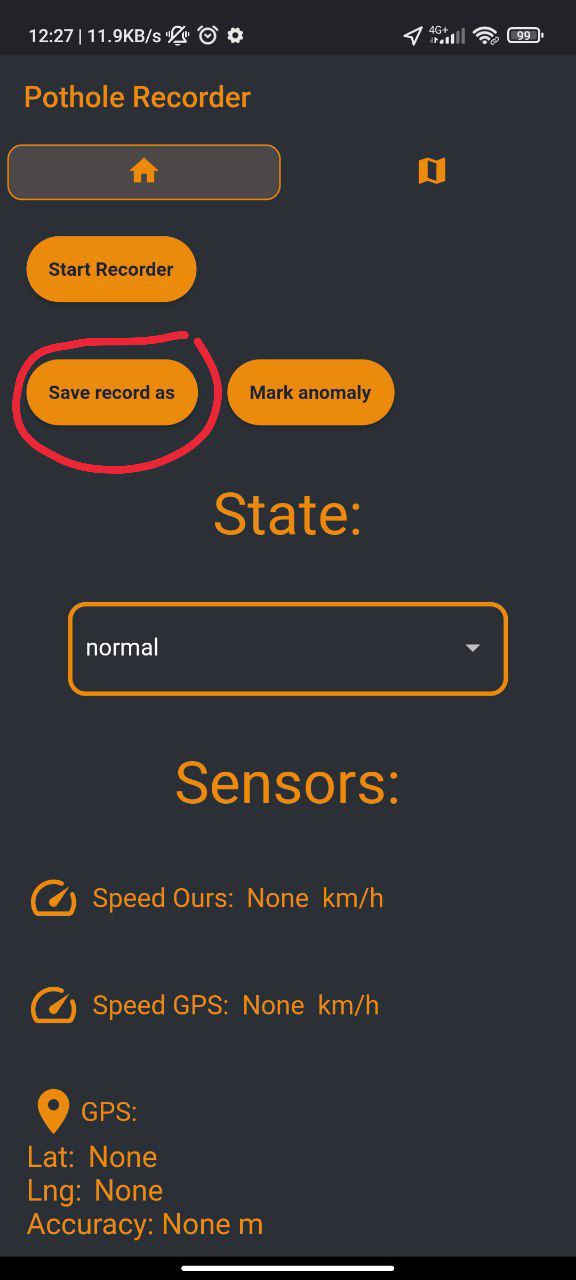
\includegraphics[scale = 0.175]{Graphics/apk_save_recording_1.jpg}
		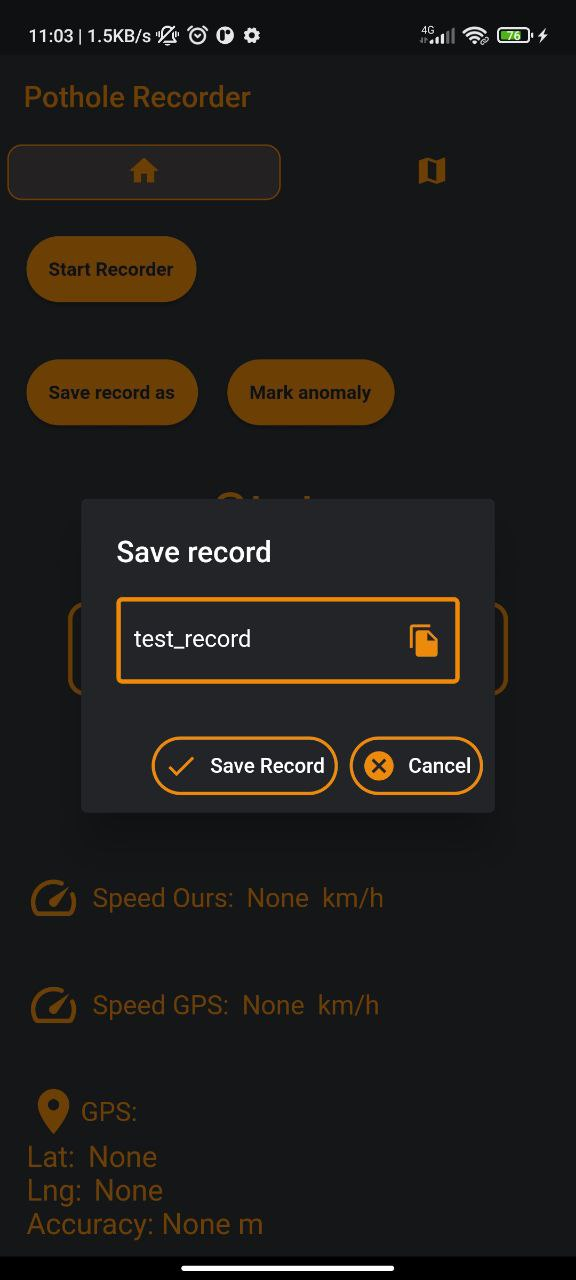
\includegraphics[scale = 0.175]{Graphics/apk_save_recording_2.jpg}
		\caption{Detener grabación y exportar}
		\label{fig:7}
	\end{figure}

	\begin{figure}[htb]
		\centering
		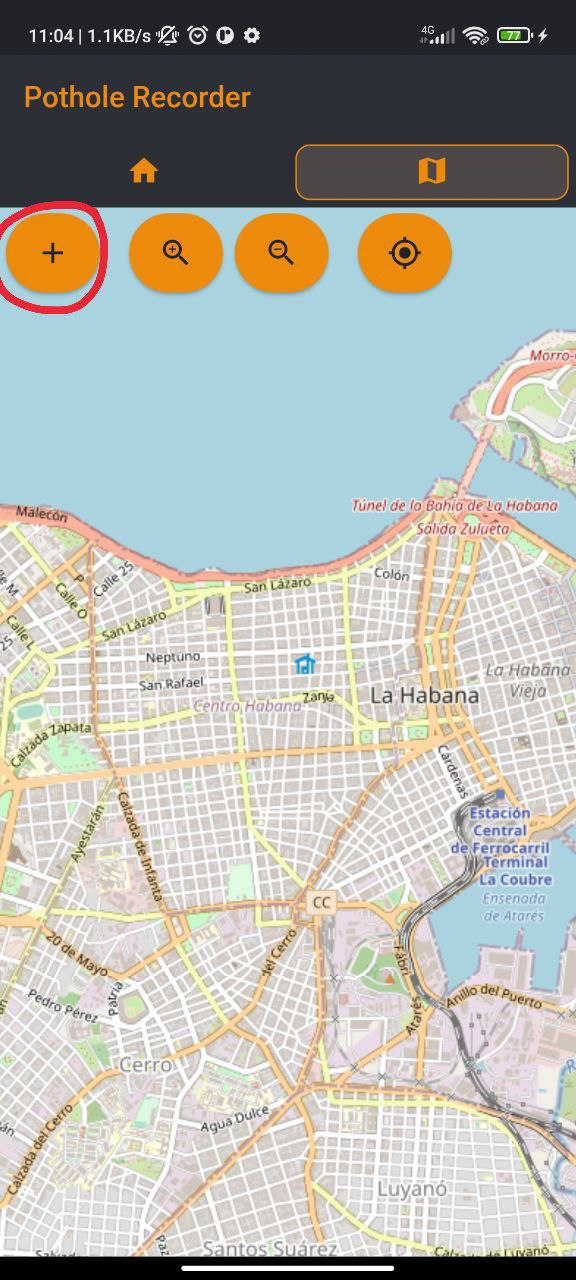
\includegraphics[scale = 0.175]{Graphics/load_marks_to_map_1.jpg}
		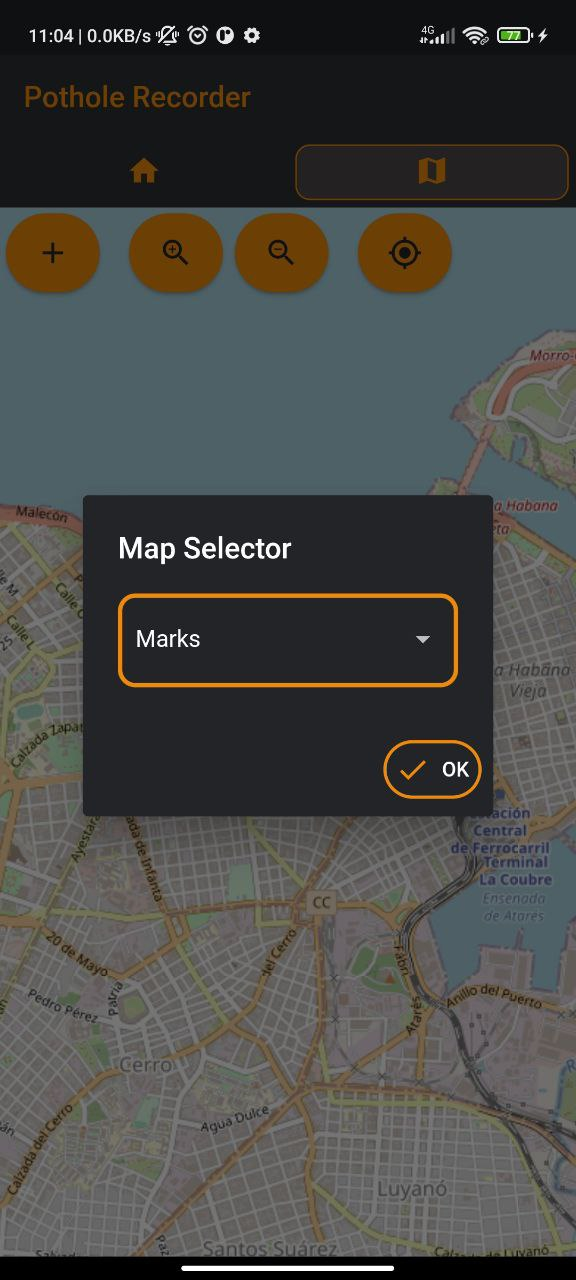
\includegraphics[scale = 0.175]{Graphics/load_marks_to_map_2.jpg}
		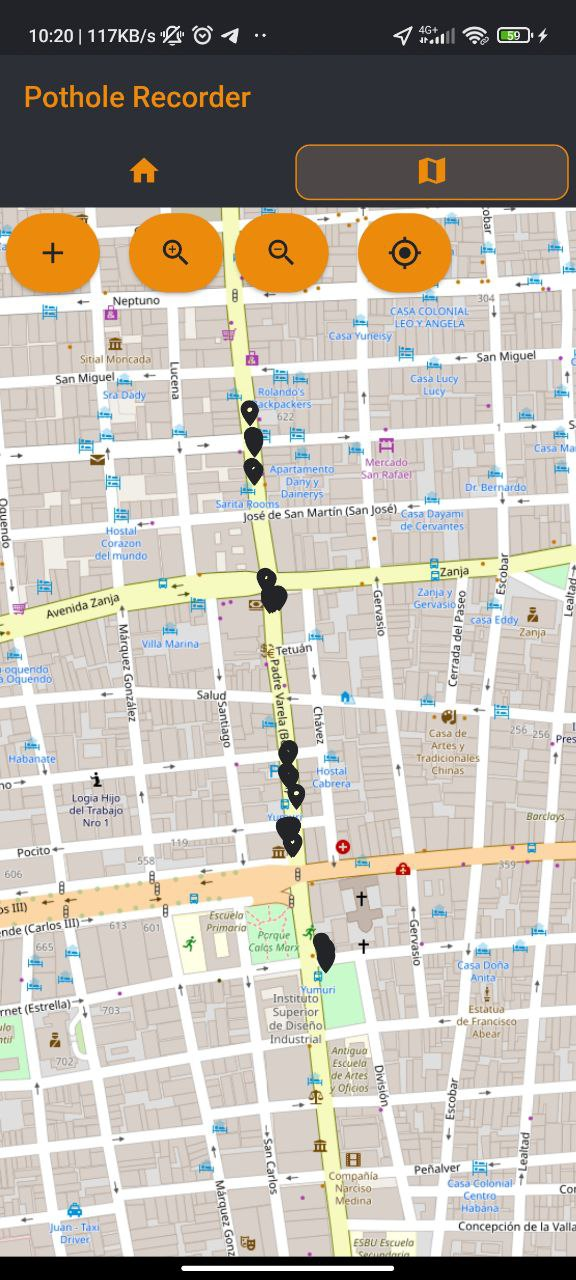
\includegraphics[scale = 0.175]{Graphics/map_marks_apk.jpg}
		\caption{Cargar marcas en el mapa de la aplicación}
		\label{fig:8}
	\end{figure}
	\newpage

	Los datos se guardan en archivos .\textbf{JSON}. Las marcas guardan \textbf{latitud}, \textbf{longitud}, \textbf{precisión} y una 
	etiqueta para indicar que en esa ubicación hay un bache. Por otro lado, las lecturas guardan \textbf{aceleración} en los 3 ejes, 
	\textbf{velocidad de giro} en los 3 ejes, \textbf{latitud}, \textbf{longitud}, \textbf{precisión}, \textbf{velocidad}, \textbf{estado}
	y \textbf{frecuencia de muestreo}. Estos datos se almacenan en el archivo temporal y en los datos una vez exportados. En este último, también 
	se guarda la duración en milisegundos, del recorrido realizado.

	La aplicación cuenta además, con una funcionalidad que permite etiquetar ciertas capturas con frases como \textbf{girar izquierda},
	\textbf{girar derecha}, \textbf{frenar} y \textbf{normal}. Con estas estiquetas, se puede registrar cuando el vehículo dobla en alguna
	esquina o cuando frena, mientras se captura la señal. Esto puede ser útil para descartar anomalías asociadas a estos eventos o
	para mostrar y analizar el comportamiento de las señales de los sensores mientras el vehículo se encuentra en alguno de estos estados
	(ver figura \ref{fig:9}).

	\begin{figure}[htb]
		\centering
		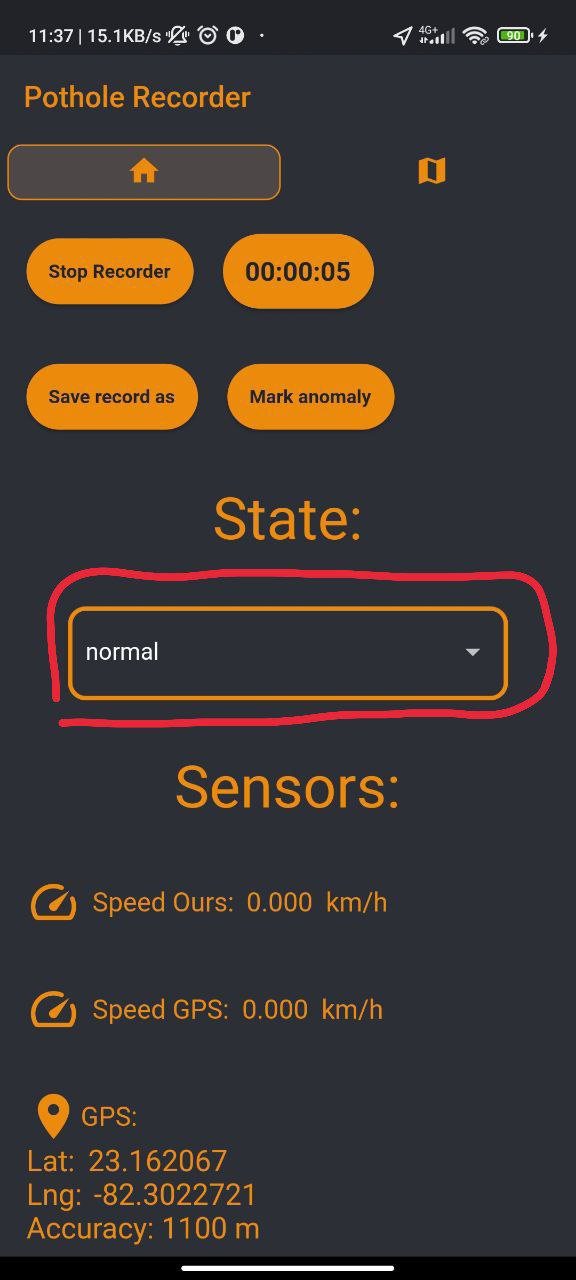
\includegraphics[scale = 0.2]{Graphics/apk_change_state_1.jpg}
		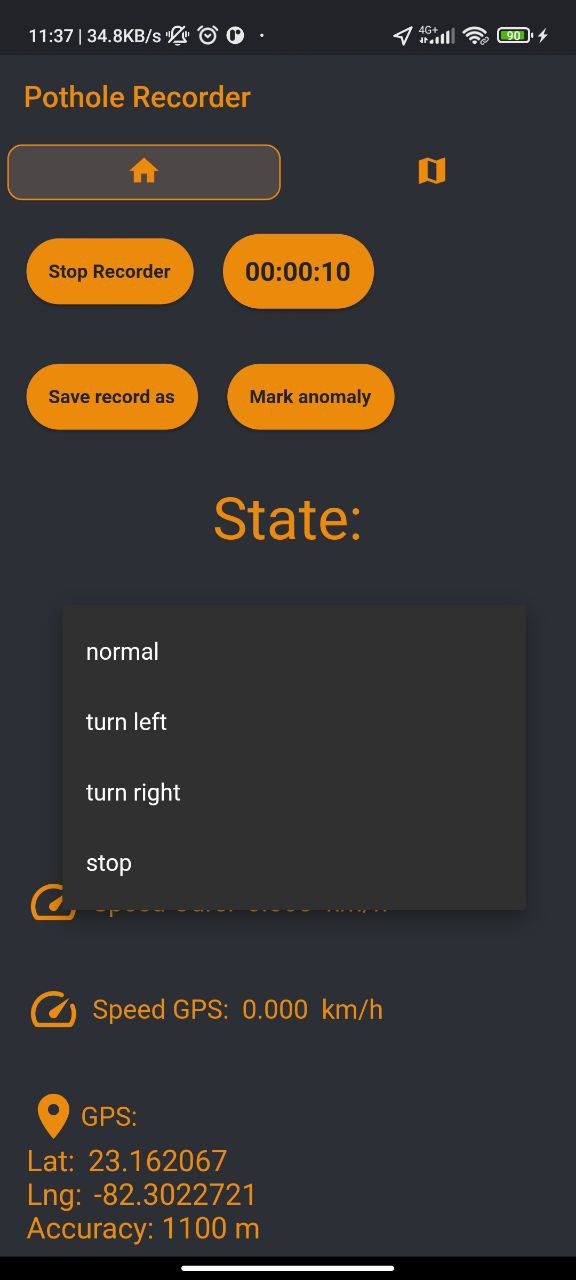
\includegraphics[scale = 0.2]{Graphics/apk_change_state_2.jpg}
		\caption{Cambiar el estado de las lecturas}
		\label{fig:9}
	\end{figure}

	\subsection{\emph{Hardware} y \emph{software} en los que se probó la aplicación}
		La aplicación se probó en dos dispositivos móviles. Un \textbf{Xiaomi Mi A2} y un \textbf{Xiaomi Redmi 10} con \textbf{Android 9} y
		\textbf{11} respectivamente. Ambos dispositivos tienen \textbf{acelerómetro}, \textbf{giroscopio} y \textbf{GPS}. El dispositivo que 
		se escogió para capturar las señales y realizar las marcas de los baches fue el \textbf{Xiaomi Redmi 10}, debido a que este tenía mejor
		precisión en las lecturas del \textbf{GPS}, las cuales se mantuvieron en un rango de 1.3 a 9 metros. En el \textbf{Xiaomi Mi A2}, las 
		lecturas del \textbf{GPS} se mantuvieron generalmente por encima de 50 metros, rara vez por debajo de esa cifra.

	\subsection{Metodología para la captura de señales}
		Primero que todo, para capturar las señales, se escogieron varias rutas de La Habana de longitud moderada. Una vez montado en un vehículo
		se colocó el dispositivo en el asiento de tal forma que su eje Y coindiera con el eje Y del vehículo y su pantalla estuviera hacia arriba.
		Apenas el vehículo comenzó a moverse, se puso la aplicación a grabar. Durante el viaje, dado que no se contaba con un objeto capaz de fijar el
		dispositivo móvil en la posición deseada, se tuvo que sostener lo mejor posible con las manos para que mantuviera la orientación. \\
		\indent Cuando el vehículo se iba a detener por alguna razón y se estaba al tanto, se cambiaba al estado de \textbf{frenar} un poco antes, para
		registrar tal evento en los datos. Lo mismo se hizo cuando el vehículo iba a doblar una esquina. Una vez terminaba el evento, se cambiaba otra
		vez a estado \textbf{normal}. Cuando el vehículo llegaba al final de la ruta planeada, se detenía el proceso de grabación y se exportaban los
		datos de dicho recorrido a un archivo .\textbf{JSON} aparte con un nombre que indentificara la ruta.

	\subsection{Metodología para marcar los baches}
		Para marcar los baches, se recorrió la misma ruta que se había seleccionado para capturar los datos, y se fueron marcando los baches. Antes 
		de realizar las marcas, se esperó un tiempo a que la precisión del \textbf{GPS} se estabilizara en un rango aceptable, preferiblemente por debajo 
	
		de los 5 metros. Las marcas se realizaron desde la acera debido al tráfico, y en la medida de lo posible un poco más cerca del bache en la calle.
		Por cada bache, se realizaron varias marcas con distinta precisión y desde distintas ubicaciones relativamente cercanas a la ubicación real del
		bache, con el objetivo de minimizar el efecto del error inherente del \textbf{GPS}. Una vez que se terminaron de marcar los baches en el recorrido
		en cuestión, se exportaba dicho archivo con un nombre similar al de las lecturas para poder relacionarlos uno con el otro a la hora de utilizarlos.

	\subsection{Error en las lecturas y las marcas}
		En las lecturas durante los recorridos existe cierto error. Esto se debe a que no se pudo fijar el dispositivo en la posición óptima y se tuvo que
		sostener con las manos, lo que sin duda alguna influye negativamente en los datos obtenidos. También, en estas lecturas así como en las marcas, hay un
		error inherente del propio \textbf{GPS}. En las marcas además, hay un error extra debido a que estas se realizaron desde la acera.

\section{Los juegos de datos}   
	Los juegos de datos que se recopilaron fueron los correspondientes a 3 recorridos hechos a lo largo de 3 rutas de la ciudad de la Habana.

	\begin{figure}[htb]
		\centering
		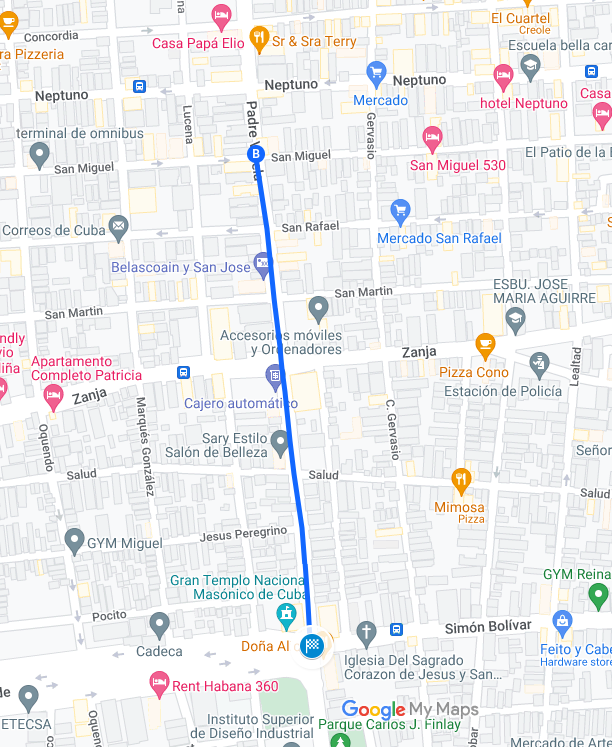
\includegraphics[scale = 0.5]{Graphics/route_1_BelascoainyReina_BelascoainySanMiguel.png}
		\caption{Ruta 1}
		\label{fig:10}
	\end{figure}

	La ruta 1 se tomó empezando en Belascoaín y Reina hasta Belascoaín y San Miguel (ver \ref{fig:10}) y tiene una longitud de 0.5 km. La ruta
	2 comienza en Egido y Arsenal y termina en Ayesteran y 19 de mayo (ver \ref{fig:11}) y tiene una longitud de 3.32 km. La ruta 3 comienza en
	Egido y Arsenal y termina en L y Jovellar (ver \ref{fig:12}) y tiene una longitud de 3.73 km.\\ \indent Se trataron de escoger rutas donde
	hubieran una cantidad importante de baches que se pudieran utilizar para el modelo.
	\newpage

	\begin{figure}[htb]
		\centering
		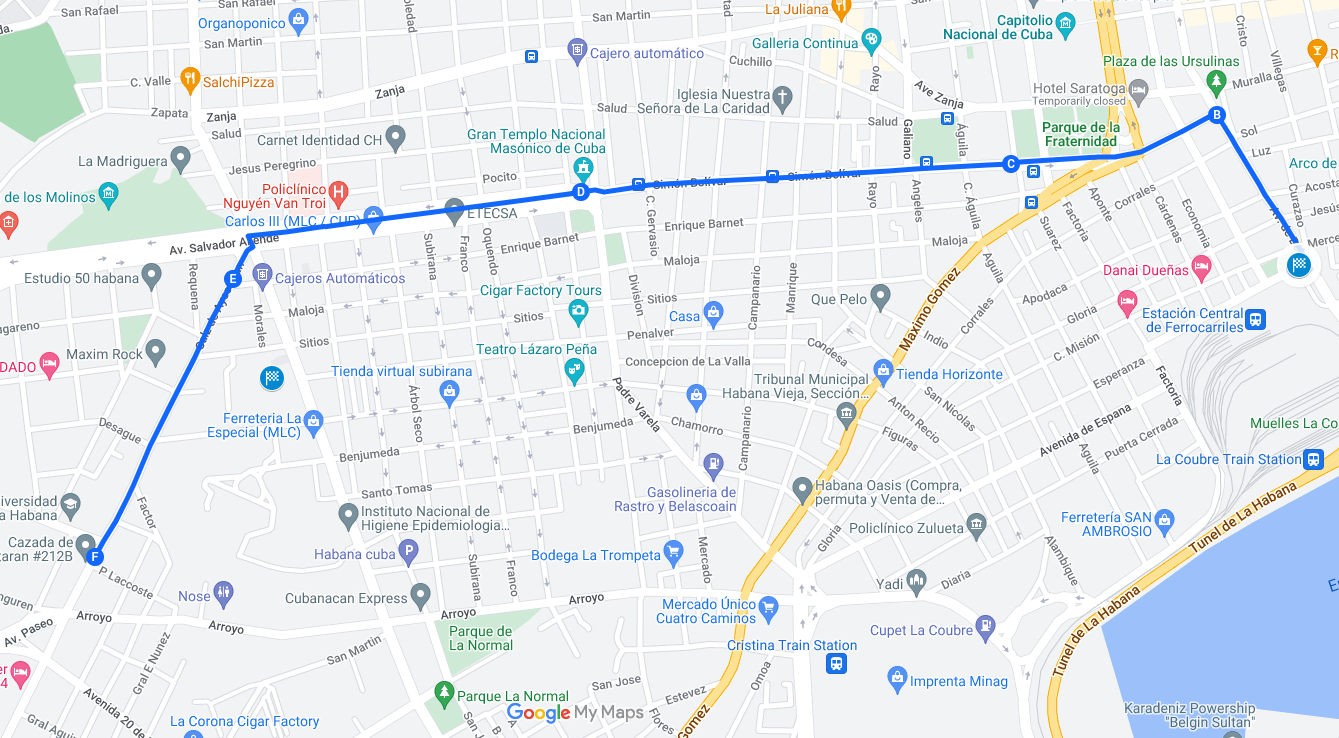
\includegraphics[scale = 0.4]{Graphics/route_2_EgidoArsenal_Ayesteran19deMayo.png}
		\caption{Ruta 2}
		\label{fig:11}
	\end{figure}

	\begin{figure}[htb]
		\centering
		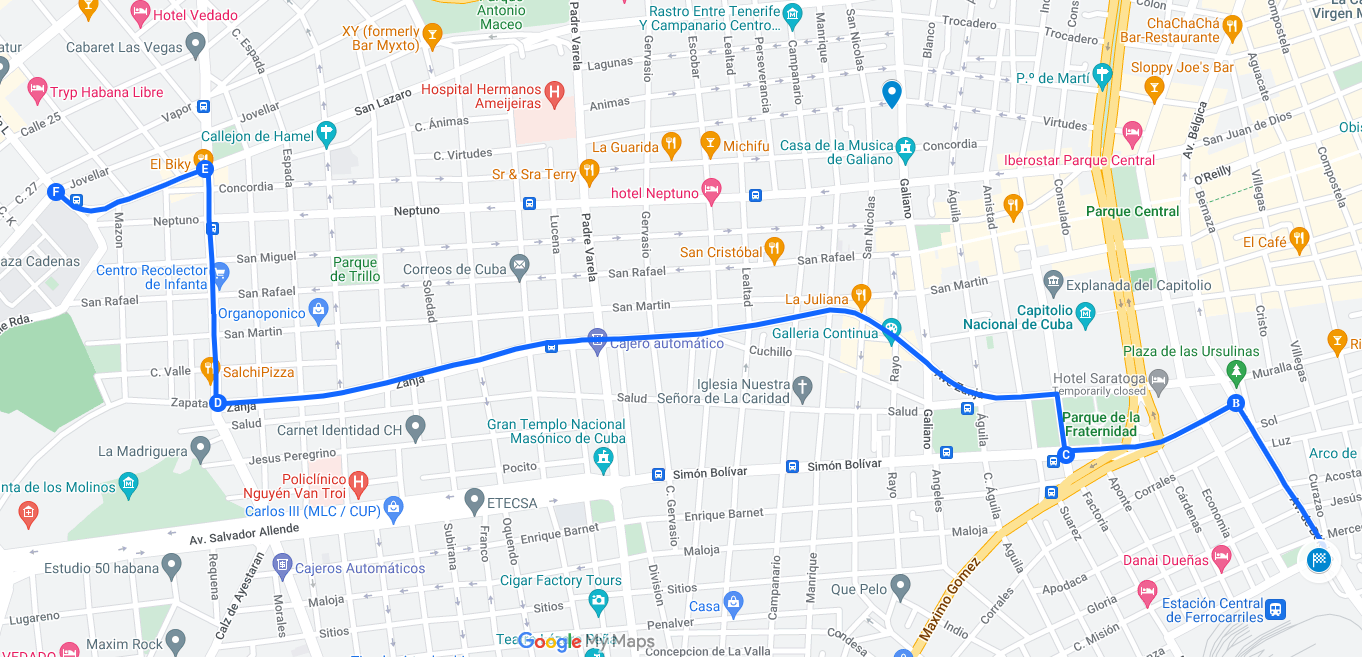
\includegraphics[scale = 0.4]{Graphics/route_3_EgidoArsenal_LyJovellarHotelColina.png}
		\caption{Ruta 3}
		\label{fig:12}
	\end{figure}

	\subsection{Detalles acerca de algunos de los baches marcados}
		En las recorridos realizados hay una gran variedad de anomalías que son baches, también hay muchas anomalías, que por sus características,
		son idénticas a un bache, como por ejemplo, una boca de alcantarilla hundida en el pavimento (ver \ref{fig:13}), que en condiciones normales no 
		tendría las mismas características (ver \ref{fig:14}). A pesar de que ambas son tapas de alcantarilla, en el primer caso las lecturas de los 
		sensores es muy probable que hayan sido similares a las de un bache.
		
		\begin{figure}[htb]
			\centering
			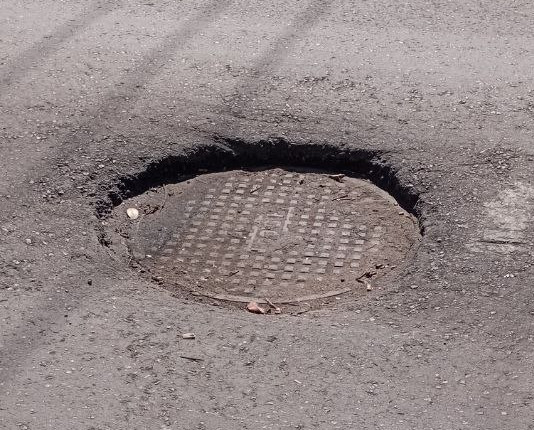
\includegraphics[scale = 0.4]{Graphics/pothole_3.jpg}
			\caption{Boca de alcantarilla hundida en el pavimento}
			\label{fig:13}
		\end{figure}

		\begin{figure}[htb]
			\centering
			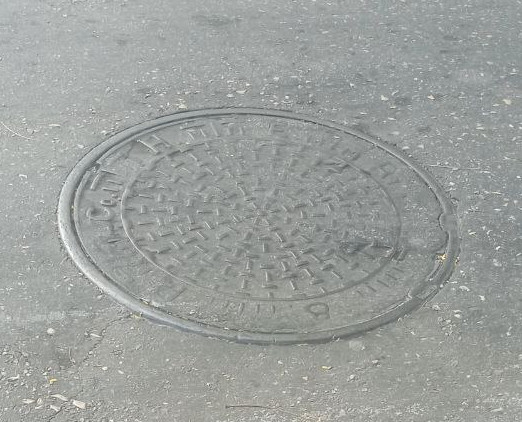
\includegraphics[scale = 0.4]{Graphics/pothole_9.jpg}
			\caption{Boca de alcantarilla}
			\label{fig:14}
		\end{figure}

		De igual forma, algunas otras tapas de alcantarillas no tiene las características que verdaderamente le corresponde como se puede ver en la
		figura \ref{fig:15}.

		\begin{figure}[htb]
			\centering
			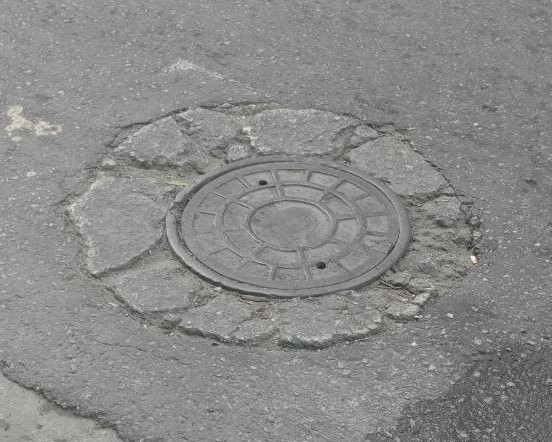
\includegraphics[scale = 0.3]{Graphics/pothole_4.jpg}
			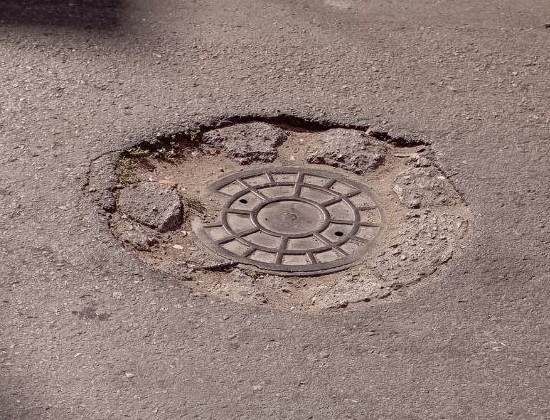
\includegraphics[scale = 0.3]{Graphics/pothole_5.jpg}
			\caption{tapas de alcantarilla con características anormales}
			\label{fig:15}
		\end{figure}

		Existen también otros objetos en la vía que no tienen las características reales y que pueden ocasionar las lecturas de los sensores sean similares
		a las de un bache como se muestra en la figura \ref{fig:16}.

		\begin{figure}[htb]
			\centering
			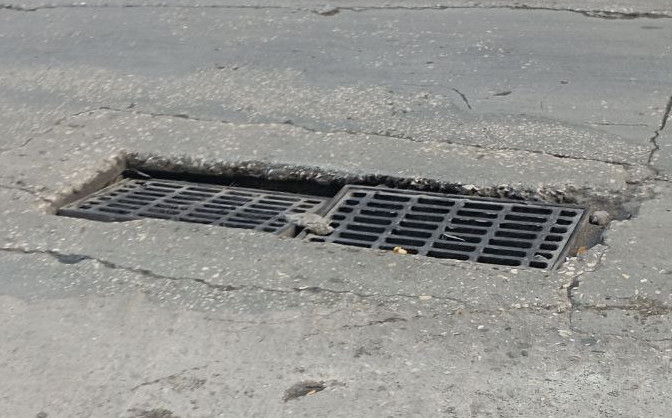
\includegraphics[scale = 0.3]{Graphics/pothole_10.jpg}
			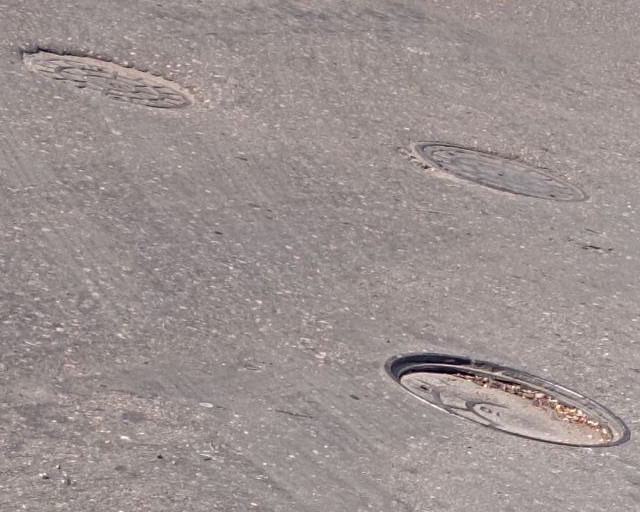
\includegraphics[scale = 0.3]{Graphics/pothole_11.jpg}
			\caption{Otros objetos en la vía con características anormales}
			\label{fig:16}
		\end{figure}

		\begin{figure}[htb]
			\centering
			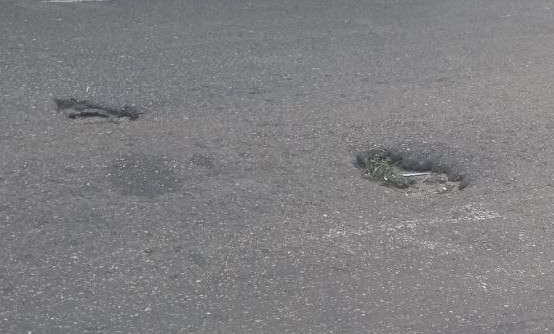
\includegraphics[scale = 0.3]{Graphics/pothole_7.jpg}
			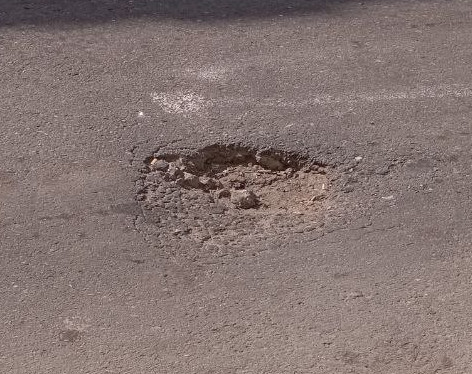
\includegraphics[scale = 0.3]{Graphics/pothole_8.jpg}
			\caption{Algunos baches de algunas de las rutas seleccionadas}
			\label{fig:17}
		\end{figure}
		\newpage

		Estas anomalías que se consideraron que podían generar lecturas	similares a las de un bache se etiqutaron como tal, al igual que las anomalías que se 
		pueden apreciar en las figuras \ref{fig:17} y \ref{fig:18}, que sí son realmente baches.

		\begin{figure}[htb]
			\centering
			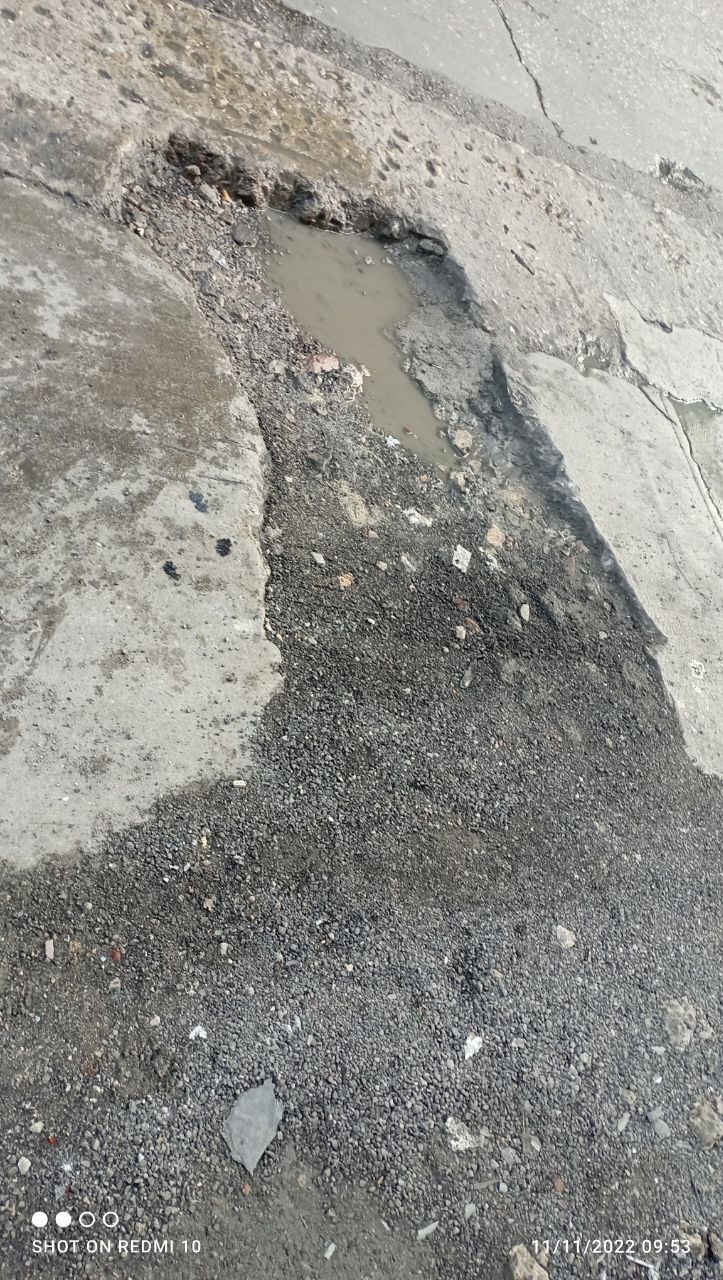
\includegraphics[scale = 0.3]{Graphics/pothole_1.jpg}
			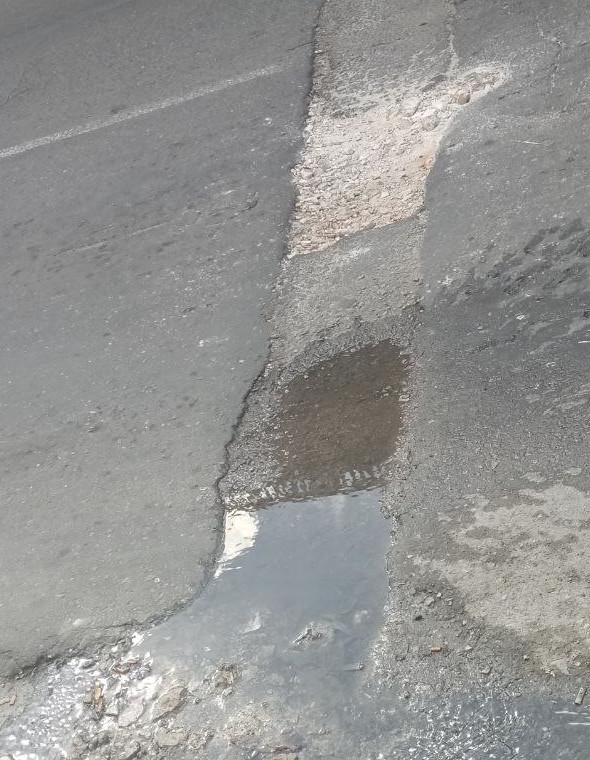
\includegraphics[scale = 0.3]{Graphics/pothole_2.jpg}
			\caption{Algunos baches de algunas de las rutas seleccionadas}
			\label{fig:18}
		\end{figure}

\section{Los modelos de aprendizaje de máquinas}
	Luego de haber recopilado los datos con la aplicación móvil, estos fueron pasados a un programa hecho en \textbf{Python 3.10.6} con el objetivo de llevar a cabo 
	la segunda fase de la propuesta. Dentro de este programa, es donde se determina que modelo de aprendizaje de máquinas se ajusta mejor al juego de datos,
	pero antes de esto fue necesario procesar los datos recolectados por la aplicación móvil y estructuralos de forma conveniente. 

	\subsection{Detalles de la estructura del juego de datos y características escogidas}
		Con el juego de datos cargado ya en el programa, se construyó un \textbf{DataFrame} de la biblioteca \textbf{pandas} donde cada columna representa
		una característica y cada fila uno de los datos recopilados. Entre las columnas de este \textbf{DataFrame} están los valores de los 3 ejes del \textbf
		{acelerómetro}, los valores de los 3 ejes del \textbf{giroscopio} y la velocidad. Estas son las primeras 7 características de nuestro juego de datos
		y son obtenidas directamente al leer los datos recopilados.\\
		\indent El resto de características, son características estadísticas generadas a partir de las 7 previamente mencionadas, y tienen como objetivo
		enriquecer el juego de datos para obtener una representación más precisa del problema que se pretende resolver. Estas características estadísticas,
		que fueron mencionadas en el capítulo anterior (ver \ref{chapter:proposal}), son computadas y agregadas como columnas al \textbf{DataFrame}.
		Luego, se agregan las columnas correspondientes a la latitud, longitud y precisión de dicha ubicación, para cada uno de los datos.\\
		\indent Finalmente, son eliminadas las lecturas donde la precisión es mayor que 10 metros, y se recomputa la latitud y longitud de cada dato con
		interpolación lineal utilizando la biblioteca \textbf{nvector}.

	\subsection{Detalles de la detección de anomalías}
		Una vez se tuvo el juego de datos completamente generado y refinado de acuerdo a las necesidades, se realizó un proceso de detección de anomalías.
		Para este proceso se probaron 6 métodos, 3 heurísticos y 3 métodos de aprendizaje de máquinas. Los 3 métodos heurísticos fueron los mencionados 
		en el capítulo previo (ver \ref{chapter:proposal}), \textbf{Z-Thresh}, \textbf{Z-Diff} y \textbf{G-Zero}. Con \textbf{Z-Thresh} debido a que 
		los valores de la aceleración en el eje Z se mantuvieron entre 9 y 10 mayormente (debido a la aceleración de la gravedad), se decidió escoger
		11 como umbral. Con \textbf{Z-Diff}, se decidió escoger 6, pues en este caso lo que se intenta es detectar cambios bruscos en los valores de
		aceleración en el eje Z y en el caso de \textbf{G-Zero} se escogió 0.8 como se recomienda en la literatura.\\
		\indent Para la detección de anomalías utilizando los métodos de aprendizaje de máquinas se utilizaron 6 de las características del \textbf
		{DataFrame}, la aceleración en los 3 ejes y la velocidad de giro en los 3 ejes. Los métodos de aprendizaje no-supervisado utilizados están
		implementados en la biblioteca \textbf{sklearn} de \textbf{Python}, específicamente en los módulos \textbf{sklearn.cluster}, donde se encuentran
		\textbf{DBSCAN} y \textbf{OPTICS}, y en \textbf{sklearn.svm}, donde se encuentra \textbf{One Class SVM}.\\
		\indent De esta forma, con cada uno de estos 6 métodos, se obtenía un \textbf{DataFrame} con los datos seleccionados como anomalías.
		Los métodos no supervisados que mejor rendimiento mostraron en general fueron \textbf{DBSCAN} y \textbf{One Class SVM} como se muestra en 
		la figura \ref{table:1}. En la tabla \ref{table:2}, se puede apreciar la media de los coeficientes de Silhouete entre todas las rutas.

		\begin{figure}[htb]
			\centering
			\begin{tabular}{llll}
			\toprule
			  Ruta\textbackslash Algoritmo &    DBSCAN &     OCSVM &     OPTICS \\
			\midrule
			  Ruta1 &  0.502849 &  0.533472 &  -0.245268 \\
			  Ruta2 &  0.659878 &  0.533707 &  -0.271357 \\
			  Ruta3 &  0.620526 &  0.509438 &  -0.238291 \\
			\bottomrule
			\end{tabular}
			\caption{Puntuación de Silhouete de cada algoritmo de detección de anomalías no-supervisado en cada ruta}
			\label{table:1}
		\end{figure}

		\begin{figure}[htb]
			\centering
			\begin{tabular}{ll}
			\toprule
			   Coeficiente de Silhouete medio & Algoritmo \\
			\midrule
			   0.594417 &    DBSCAN \\
			   0.525539 &     OCSVM \\
			  -0.251639 &    OPTICS \\
			\bottomrule
			\end{tabular}
			\caption{Puntuación de Silhouete media de cada algoritmo de detección de anomalías no-supervisado}
			\label{table:2}
		\end{figure}

		Como se puede apreciar, \textbf{OPTICS} tuvo una puntuación incluso por debajo de 0, lo que indica que los clusters se asignaron de 
		forma errónea. Por esta razón se optó por removerlo del \emph{pipeline} de la propuesta. También se recopiló información acerca de la
		cantidad de anomalías detecto cada algoritmo (ver tabla \ref{table:3}). También se eliminó del \emph{pipeline} \textbf{G-Zero}
		,pues se consideró que no detectó suficientes anomalías, se supone que la frecuencia de muestreo a la que se realizaron las capturas
		fue demasiado baja, y debido a esto no fue posible obtener los datos representativos del instante en el que el vehículo está en caída libre.

		\begin{figure}[htb]
			\centering
			\begin{tabular}{ll}
				\toprule
				 Algoritmo &  Número de Anomalías \\
				\midrule
				    DBSCAN &                  134 \\
				     OCSVM &                  446 \\
				    z-diff &                  181 \\
				   z-tresh &                   95 \\
				    g\_zero &                    0 \\
				\bottomrule
			\end{tabular}
			\caption{Número de anomalías detectadas por cada algoritmo}
			\label{table:3}
		\end{figure}

		Los hiperparámetros de los métodos de detección de anomalías que se probaron para determinar la mejor configuración se muestran en las tablas 
		\ref{table:4}, \ref{table:5} y \ref{table:6}.

		\begin{figure}[htb]
			\centering
			\begin{tabular}{ll}
				\toprule
				                                          eps &                                  min\_samples \\
				\midrule
				  0.05, 0.1, ..., 0.95, 0.99 &  15, 20, ..., 60, 65 \\
				\bottomrule
			\end{tabular}
			\caption{Hyperparámetros con los que se probó \textbf{DBSCAN}}
			\label{table:4}
		\end{figure}
		
		\begin{figure}[htb]
			\centering
			\begin{tabular}{ll}
				\toprule
				                                            gamma &                                                 nu \\
				\midrule
				  scale, 0.00001, 0.0001, 0.001, 0.01, 0.1, 1, 10 &  0.05, 0.1, ..., 0.95, 0.99 \\
				\bottomrule
			\end{tabular}
			\caption{Hyperparámetros con los que se probó \textbf{One Class SVM}}
			\label{table:5}
		\end{figure}
		
		\begin{figure}[htb]
			\centering
			\begin{tabular}{lll}
				\toprule
				 cluster\_method &                                      metric &                                        min\_samples \\
				\midrule
				     xi, dbscan &  minkowski, euclidean, canberra, braycurtis &  5, 10, ..., 60, 65 \\
				\bottomrule
			\end{tabular}
			\caption{Hyperparámetros con los que se probó \textbf{OPTICS}}
			\label{table:6}
		\end{figure}

	\subsection{Detalles del proceso de etiquetado}
		Con cada uno de los juegos de datos obtenidos por cada uno de los métodos utilizados para detectar anomalías, se llevó a cabo
		el proceso de etiquetado para indentificar que anomalía es un bache. Esto, como se mencionó en el capítulo anterior(ver \ref{chapter:proposal}),
		se llevó a cabo utilizando el conjunto de marcas correspondientes a la serie temporal de la cual se extrajeron las anomalías. De esta manera, se
		le asigna una etiqueta a una anomalía indicando que es bache, si existe una marca en el conjunto de marcas que se encuentre en un radio de 10
		metros. Se consideró 10 metros, debido al error que mantuvo el dispositivo que se utilizó para la captura de los datos durante el proceso de
		recopilación.\\
		\indent Para computar la distancia se utilizó la fórmula de \textbf{Haversine}, que se utiliza para calcular la distancia entre dos puntos sobre la
		superficie de una esfera utilizando coordenadas de latitud-longitud. Debido a que la \textbf{Tierra} no es una esfera perfecta, tiene distintos radios, que
		van desde 6356.752 km en los polos hasta 6378.137 km en el Ecuador. A causa de esto, es imposible calcular exactamente la distancia entre 2 puntos
		con esta fórmula, pero el error al hacerlo es de un 0.5\%, por lo que es bastante despreciable. El radio de la esfera que se consideró para este
		cómputo fue de 6371 km.\\

	\subsection{Detalles de la selección de características}
		Por cada juego de anomalías etiquetadas, como ya se mencionó en el capítulo previo (ver \ref{chapter:proposal}), se llevó a cabo un proceso
		de selección de características con varios métodos, para escoger cuales de estas representan mejor el problema que se pretende resolver.
		Antes de esto se eliminaron características que se consideraron no aportan información acerca de si una anomalía es bache o no, como por ejemplo:
		la velocidad, la latitud, la longitud y la precisión del \textbf{GPS}.\\
		\indent El clasificador que se utilizó para estimar dichas características en el proceso de selección fue un \emph{Random Forest}, y fue
		utilizado el que brinda el módulo \textbf{sklearn.ensembles} de la bibliotea \textbf{sklearn}. Cada vez que se corrían los métodos de selección
		de características se almacenó la información de que características se escogieron, de esta forma, luego se pudo analizar en general que
		características fueron más escogidas. A dichos métodos se les pasaba el número de características a seleccionar. Las cantidades de características
		con que las que se probaron fueron: 3, 6 y 9.\\
		% ------------ Poner tabla de características más utilizadas ---------------- %

	\subsection{Detalles de la selección de modelo}
		Una vez el algoritmo de selección de características terminaba, se generaba un nuevo \textbf{DataFrame} con esas únicas columnas como datos,
		y fue con este juego de datos que se pasaba a la fase de selección de modelo. En esta, se llevó a cabo un extenso proceso en el cual se buscó
		el mejor algoritmo con la mejor configuración de hiperparámetros para ese juego de datos. Los varios algoritmos que se probaron fueron
		mencionados en el capítulo anterior (ver \ref {chapter:proposal}).\\
		\indent Para llevar a cabo esta fase de la propuesta se utilizó la biblioteca \textbf{sklearn} de \textbf{Python}.
		Para los modelos, se utilizaron los módulos \textbf{sklearn.svm}, \textbf{sklearn.trees}, \textbf{sklearn.linear\textunderscore models},
		\textbf{sklearn. ensembles} y \textbf{sklearn.neighbors}, que permiten utilizar los métodos de aprendizaje supervisado \textbf{SVM}, \emph
		{Decision Trees}, regresión logística, \emph{Random Forest} y \textbf{KNN} respectivamente. Para separar los datos en conjunto de entrenamiento
		y de prueba se utilizó el método \textbf{train\textunderscore test\textunderscore split} del módulo \textbf{sklearn.model\textunderscore
		selection}.\\
		\indent Del mismo módulo se utilizaron los objetos \textbf {RepeteadStratifiedKFold} y \textbf{GridSearchCV} para realizar validación cruzada y
		para selección de hiperparámetros respectivamente. La métrica utilizada fue \emph{F1 score}, para esto utilizamos el método \textbf{f1\textunderscore
		score} del módulo \textbf{sklearn.metrics}. De esta forma, para cada uno de los 5 métodos utilizados, se pudo determinar la mejor configuración
		de hiperparámetros, realizar la validación cruzada y obtener el mejor modelo para la fase de prueba, utilizando la métrica seleccionada. A \textbf{
		RepeteadStratifiedKFold} se le pasaron argumentos para realizar 5-Fold 30 veces.

		\subsubsection{Conjuntos de hiperparámetros}
			A continuación se muestran las 5 tablas, 1 por cada método, con los hiperparámetros entre los cuales el \textbf{GridSearchCV} seleccionó.\\

			\begin{figure}[ht!]
				\centering
				\begin{tabular}{llll}
					\toprule
						   n\_neighbors &            weights &                  algorithm &       leaf\_size \\
					\midrule
					 3, 5, 7, 9, 11 &  uniform, distance &  brute, kd\_tree, ball\_tree &  20, 30, 40, 50 \\
					\bottomrule
				\end{tabular}
				\caption{Hiperparámetros \textbf{KNN}}
				\label{table:7}
			\end{figure}

			\begin{figure}[ht!]
				\centering
				\begin{tabular}{llll}
					\toprule
							criterion &        splitter &           max\_depth &      max\_features \\
					\midrule
					  entropy, gini &  best, random &  3, 4, 5, 6, None &  sqrt, log2, None \\
					\bottomrule
				\end{tabular}
				\caption{Hiperparámetros \emph{Decision Tree}}
				\label{table:8}
			\end{figure}
			
			\begin{figure}[ht!]
				\centering
				\begin{tabular}{llll}
					\toprule
					     n\_estimators &        criterion &          max\_depth &  max\_features \\
					\midrule
					  100, 120, 180 &  entropy, gini &  10,  13, 16, 20 &  log2, sqrt \\
					\bottomrule
				\end{tabular}
				\caption{Hiperparámetros \emph{Randon Forest}}
				\label{table:9}
			\end{figure}

			\begin{figure}[ht!]
				\centering
				\begin{tabular}{lllll}
					\toprule
					 penalty &                       tol &                   C &         solver &        max\_iter \\
					\midrule
					    l2 &  1e-3, 1e-4, 1e-5, 1e-6 &  1, 10, 100, 1000 &  lbfgs, saga &  100, 500, 1000 \\
					\bottomrule
				\end{tabular}
				\caption{Hiperparámetros regresión logística}
				\label{table:10}
			\end{figure}
			\newpage

			\begin{figure}[ht!]
				\centering
				\begin{tabular}{llll}
					\toprule
					      C & kernel &          gamma &  probability \\
					\midrule
					  100 &  rbf &  0.01, 0.001 &         True \\
					\bottomrule
				\end{tabular}
				\caption{Hiperparámetros \textbf{SVM}}
				\label{table:11}
			\end{figure}
